\documentclass[conference]{IEEEtran}
\usepackage{cite}
\usepackage{amsmath,amssymb,amsfonts}
\usepackage{algorithmic}
\usepackage{graphicx}
\usepackage{textcomp}
\usepackage{xcolor}
\usepackage{hyperref}
\usepackage{tikz}
\usetikzlibrary{positioning, arrows.meta, shadows}

\begin{document}

\title{Trustless Notes: A Zero-Knowledge Encrypted Note-Taking Application}

\author{
\begin{tabular}{cc}
\begin{tabular}{c}
\textbf{Srinidhi H}\\
Dept. of Computer Science and Engineering\\
RV College of Engineering\\
srinidhih.cs23@rvce.edu.in
\end{tabular}
&
\begin{tabular}{c}
\textbf{Srikar Rao H M}\\
Dept. of Computer Science and Engineering\\
RV College of Engineering\\
srikarraoh.cs23@rvce.edu.in
\end{tabular}
\\[1cm]
\begin{tabular}{c}
\textbf{Suraj Sreedhara}\\
Dept. of Computer Science and Engineering\\
RV College of Engineering\\
surajsreedhara.cs23@rvce.edu.in
\end{tabular}
&
\begin{tabular}{c}
\textbf{Prof. Savitri Kulkarni}\\
Assistant Professor\\
Dept. of Computer Science and Engineering\\
RV College of Engineering\\
savitrikulkarni@rvce.edu.in
\end{tabular}
\end{tabular}
}

\maketitle

\begin{abstract}
Trustless Notes is a zero-knowledge, end-to-end encrypted note-taking application that ensures the server storing user data is architecturally incapable of reading it. The system leverages the Web Cryptography API to perform all encryption and decryption exclusively on the client side, with the server storing only ciphertext, initialization vectors, salts, and wrapped cryptographic keys. Authentication follows a challenge-response protocol using PBKDF2-derived keys where the password never leaves the browser. Note sharing is implemented through ECDH P-256 key exchange combined with HKDF-derived symmetric keys, allowing selective sharing without revealing the master password or other note contents. An integrated security simulator demonstrates resilience against database breaches, password leaks, cookie forgery, and service key compromises. The application is built using Next.js with Supabase providing PostgreSQL-based relational storage and object storage for encrypted file attachments.
\end{abstract}

\begin{IEEEkeywords}
Zero-Knowledge Architecture, End-to-End Encryption, Web Cryptography, Client-Side Encryption, PBKDF2, AES-256-GCM, ECDH P-256, Network Security, Privacy-Preserving Systems
\end{IEEEkeywords}

\section{Introduction}

Cloud-based applications have become integral to modern life, with users entrusting personal data to services ranging from email and document editing to note-taking and file storage. These services typically operate on a trust-based model where the service provider has full access to user data, relying on organizational policies and legal agreements rather than technical guarantees to protect privacy. A compromised server, malicious insider, or government subpoena can expose all user data stored on such platforms.

Trustless Notes addresses this fundamental security challenge by implementing a \textbf{zero-knowledge architecture}---the server is architecturally incapable of reading user data. All cryptographic operations---key derivation, encryption, decryption, and key exchange---are performed exclusively on the client side using the Web Cryptography API, a standards-compliant interface available in all modern browsers. The server stores only ciphertext, initialization vectors (IVs), salts, and wrapped cryptographic keys, none of which can recover plaintext without the user's password-derived key that never leaves the browser.

\section{Features and Significance}

Trustless Notes implements a comprehensive set of security features that collectively ensure user data privacy even in the event of server compromise. Each feature addresses a specific vulnerability present in conventional cloud applications.

\subsection{Zero-Knowledge Authentication}

Conventional web applications authenticate users by transmitting a password (or its hash) to the server, which then compares it against a stored hash. This approach has two fundamental weaknesses: the server can verify passwords directly, and a database breach exposes password hashes to offline cracking. Trustless Notes replaces this with a sentinel-based challenge-response protocol. A random sentinel value is encrypted with the user's password-derived key on signup, and its hash is stored server-side. On sign-in, the server returns the encrypted sentinel; only someone with the correct password can decrypt it and prove their identity. The server never sees the password and cannot verify it directly. This design is critically important because it eliminates the server as an attack vector for credential theft---even a full database breach yields only encrypted sentinels that are useless without the corresponding password.

\subsection{Client-Side Encryption with Non-Extractable Keys}

All encryption and decryption occurs in the browser using keys that are created with the non-extractable flag. This means the raw key material can never be exported from the Web Cryptography API, even by JavaScript running in the same page. An attacker who achieves cross-site scripting (XSS) execution cannot exfiltrate the key because it exists only as an opaque handle in browser memory. This is a significant improvement over JavaScript cryptography libraries where keys are represented as byte arrays that can be accessed, logged, or transmitted by any script on the page.

\subsection{Per-Note Key Independence}

Every note is encrypted with its own unique AES-256-GCM key, which is then wrapped (encrypted) by the user's master derived key before storage. This indirection provides two critical benefits. First, it enables password rotation---a user can change their password by re-wrapping all note keys with a new derived key, without re-encrypting any note content. Second, it enables selective sharing---a specific note key can be wrapped for a recipient without exposing any other notes. In a conventional system where all data is encrypted with a single key, sharing one item would require sharing the master key, compromising all other data.

\subsection{Cryptographic Note Sharing}

Note sharing in conventional end-to-end encrypted systems often requires the server to manage key distribution, creating a potential point of compromise. Trustless Notes implements sharing through Elliptic Curve Diffie-Hellman (ECDH) key exchange over the P-256 curve. Each user generates an ECDH keypair at signup; the public key is stored openly on the server, while the private key is encrypted with the user's derived key. To share a note, the sender computes an ECDH shared secret using their private key and the recipient's public key, then derives a symmetric AES-256-GCM key via HKDF to wrap the note key. The server mediates the exchange---it stores the re-wrapped key---but cannot derive the shared secret because it has access to neither user's unencrypted private key. This ensures that the server cannot grant itself access to shared content.

\subsection{Anti-Enumeration and Session Security}

The sign-in endpoint implements anti-enumeration by returning indistinguishable responses for both valid and invalid usernames. The response size, structure, and timing are identical, preventing attackers from determining which usernames are registered on the system. Session state is maintained through HMAC-SHA256 signed cookies that provide tamper-proof authentication without exposing sensitive credentials. The signature is verified in constant time on every request, preventing timing side-channel attacks.

\section{System Architecture}

Trustless Notes follows a three-tier client-server architecture with a clear security boundary enforced by client-side encryption.

\begin{figure}[htbp]
\centering
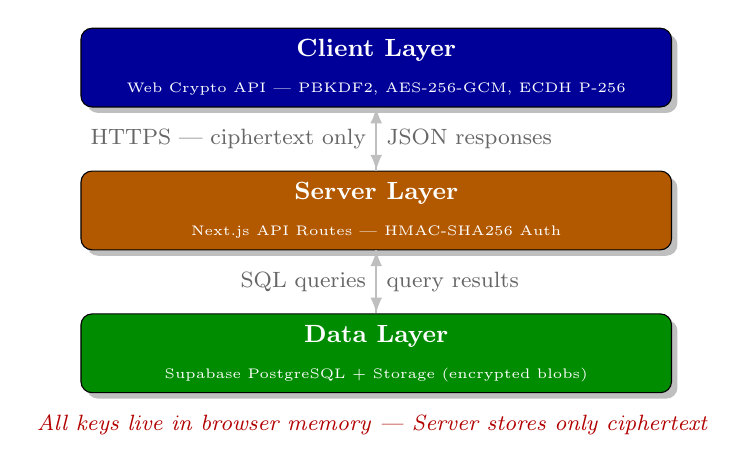
\begin{tikzpicture}[
  box/.style={draw, rounded corners=4pt, minimum width=7.5cm, minimum height=1.0cm, font=\small\bfseries, align=center, text=white},
  detail/.style={font=\footnotesize, align=center, text=gray!80!black},
  arrow/.style={-{Latex[length=2mm]}, thick, draw=gray!50},
  seclabel/.style={font=\footnotesize\itshape, text=red!70!black, align=center}
]

  % Client Layer
  \node[box, fill=blue!60!black, drop shadow] (client) {
    Client Layer \\[2pt]
    {\normalfont\tiny Web Crypto API --- PBKDF2, AES-256-GCM, ECDH P-256}
  };

  % Server Layer
  \node[box, fill=orange!70!black, drop shadow, below=0.8cm of client] (server) {
    Server Layer \\[2pt]
    {\normalfont\tiny Next.js API Routes --- HMAC-SHA256 Auth}
  };

  % Data Layer
  \node[box, fill=green!55!black, drop shadow, below=0.8cm of server] (data) {
    Data Layer \\[2pt]
    {\normalfont\tiny Supabase PostgreSQL + Storage (encrypted blobs)}
  };

  % Arrows
  \draw[arrow] (client.south) -- node[left, detail] {HTTPS --- ciphertext only} (server.north);
  \draw[arrow] (server.north) -- node[right, detail] {JSON responses} (client.south);
  \draw[arrow] (server.south) -- node[left, detail] {SQL queries} (data.north);
  \draw[arrow] (data.north) -- node[right, detail] {query results} (server.south);

  % Security annotation
  \node[seclabel, below=0.15cm of data.south] {
    All keys live in browser memory --- Server stores only ciphertext
  };

\end{tikzpicture}
\caption{Three-tier zero-knowledge architecture.}
\label{fig:architecture}
\end{figure}

\textbf{Client Layer (Browser):} The React application serves as the execution environment for all cryptographic operations. The user's derived key exists exclusively as a non-extractable CryptoKey object in browser memory. In-memory state management ensures that all sensitive data---decrypted note contents, cryptographic keys, and session information---is automatically cleared when the browser tab is closed, with no persistence to localStorage or sessionStorage.

\textbf{Server Layer:} RESTful API endpoints handle data persistence and retrieval but operate exclusively on ciphertext. The server has no access to encryption keys and no decryption capability. HMAC-SHA256 signed cookie verification is performed on every authenticated request. The server's role is limited to access control (verifying note ownership and sharing relationships) and data mediation.

\textbf{Data Layer:} A PostgreSQL database stores encrypted artifacts including ciphertext, IVs, salts, and wrapped keys. Object storage handles encrypted file attachment blobs. The data layer is purely passive---it provides storage and retrieval without any cryptographic processing capability.

\section{Cryptographic Protocol}

\subsection{PBKDF2 Key Derivation}

When the user creates an account, the browser generates a cryptographically random 16-byte salt using a cryptographically secure random number generator. The password is combined with this salt using PBKDF2 with HMAC-SHA256 for 200,000 iterations to produce a 256-bit AES-GCM key. The key is created with the non-extractable flag, meaning it can never be exported from the Web Cryptography API as raw bytes.

\[
\text{Password} + \text{Salt} \xrightarrow{\text{PBKDF2(200000, SHA-256)}} \text{Derived Key}
\]

The iteration count of 200,000 imposes a significant computational cost on brute-force attacks---each password guess requires 200,000 SHA-256 hash computations---while maintaining acceptable user experience (typically 500--1500ms on modern hardware). The salt ensures that identical passwords produce different derived keys across users, preventing precomputation attacks.

\subsection{Sentinel-Based Authentication Protocol}

The authentication protocol eliminates password transmission through a two-phase challenge-response mechanism.

\begin{figure}[htbp]
\centering
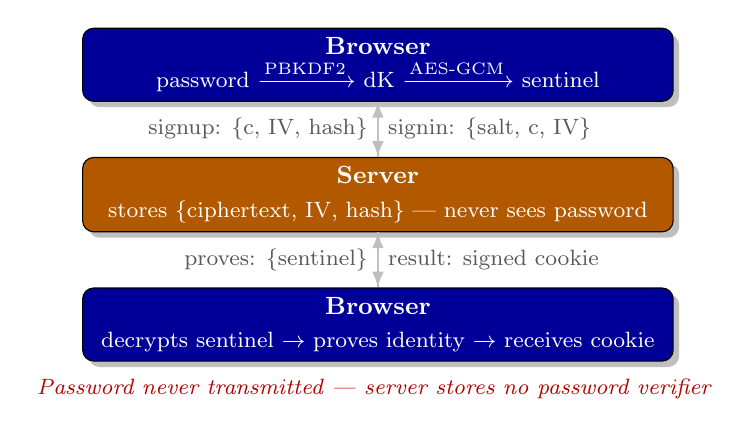
\begin{tikzpicture}[
  box/.style={draw, rounded corners=4pt, minimum width=7.5cm, minimum height=0.9cm, font=\small\bfseries, align=center, text=white},
  arrow/.style={-{Latex[length=2mm]}, thick, draw=gray!50},
  label/.style={font=\footnotesize, align=center, text=gray!70!black},
]

  % Browser
  \node[box, fill=blue!60!black, drop shadow] (browser) {
    Browser \\[1pt]
    {\normalfont\footnotesize password $\xrightarrow{\text{PBKDF2}}$ dK $\xrightarrow{\text{AES-GCM}}$ sentinel}
  };

  % Server
  \node[box, fill=orange!70!black, drop shadow, below=0.7cm of browser] (server) {
    Server \\[1pt]
    {\normalfont\footnotesize stores \{ciphertext, IV, hash\} --- never sees password}
  };

  % Signup arrow
  \draw[arrow] (browser.south) -- node[left, label] {signup: \{c, IV, hash\}} (server.north);

  % Signin reverse arrow
  \draw[arrow] (server.north) -- node[right, label] {signin: \{salt, c, IV\}} (browser.south);

  % Second browser node for signin response
  \node[box, fill=blue!60!black, drop shadow, below=0.7cm of server] (browser2) {
    Browser \\[1pt]
    {\normalfont\footnotesize decrypts sentinel $\rightarrow$ proves identity $\rightarrow$ receives cookie}
  };

  \draw[arrow] (server.south) -- node[left, label] {proves: \{sentinel\}} (browser2.north);
  \draw[arrow] (browser2.north) -- node[right, label] {result: signed cookie} (server.south);

  % Security annotation
  \node[font=\footnotesize\itshape, text=red!70!black, align=center, below=0.1cm of browser2.south] {
    Password never transmitted --- server stores no password verifier
  };

\end{tikzpicture}
\caption{Sentinel-based authentication. The password never leaves the browser; the server stores only encrypted sentinel artifacts for challenge-response verification.}
\label{fig:auth_flow}
\end{figure}

This design ensures that the server cannot verify passwords directly, cannot determine whether a username exists from the sign-in response, and cannot authenticate as the user without client-side proof of key knowledge.

\subsection{Per-Note Key Wrapping}

Each note has its own randomly generated AES-256-GCM key. The note key encrypts the title and content separately, with each encryption operation using a fresh random IV. The note key is then wrapped (encrypted) by the user's derived key before being sent to the server. This indirection provides two critical properties:
\begin{itemize}
    \item \textbf{Key independence:} Compromising one note's key does not compromise other notes.
    \item \textbf{Re-keying support:} Changing the master password requires only re-wrapping all note keys, not re-encrypting any note content.
\end{itemize}

\subsection{ECDH Key Exchange for Sharing}

Note sharing uses Elliptic Curve Diffie-Hellman (ECDH) over the P-256 curve. Each user generates an ECDH keypair at signup. The public key is stored openly on the server; the private key is encrypted with the user's derived key before storage.

On signup, each user generates an ECDH keypair. The public key is stored in plaintext on the server and is publicly fetchable. The private key is encrypted with the user's derived key before storage. To share a note, the sender fetches the recipient's public key, decrypts their own ECDH private key, and computes:

\[
\text{SharedSecret} = \text{PrivateKey}_{\text{Sender}} \times \text{PublicKey}_{\text{Recipient}}
\]

This shared secret is passed through HKDF with the note ID as salt to produce a symmetric AES-256-GCM key. The note key is unwrapped from the sender's derived key, re-wrapped with this HKDF-derived key, and stored on the server. The recipient reverses the process: they decrypt their own ECDH private key, compute the same shared secret using the sender's public key, derive the same HKDF key, and unwrap the note key. The server cannot derive the shared secret because it lacks access to either user's unencrypted ECDH private key.

\section{Security Simulator}

A central contribution of this work is the integrated educational security simulator, which provides transparent, verifiable demonstration of the system's security properties. The simulator implements four interactive attack scenarios at a dedicated route within the application. Unlike the main application where cryptographic keys are non-extractable for security, the simulator reimplements all cryptographic operations with extractable keys specifically for display purposes, allowing users to inspect intermediate values---keys, ciphertexts, and plaintexts---that would normally be invisible.

\subsection{Simulator Architecture and Design}

The simulator presents each attack scenario as a step-by-step visual narrative. A typewriter-style terminal component introduces the attack context, establishing the threat model and attacker capabilities. Interactive visual components then demonstrate each stage of the attack, from initial access through attempted exploitation. After each step, the simulator shows the cryptographic state---what the attacker has obtained versus what they would need---making it visually clear why the attack fails.

Each scenario concludes with an analysis section that summarizes the cryptographic guarantees preventing the attack. The simulator uses a distinct dark theme with hacker-aesthetic styling, clearly differentiated from the main application interface to avoid confusion between simulated and real cryptographic operations.

\subsection{Scenario 1: Database Leak}

This scenario simulates an attacker gaining unauthorized read access to the database. The simulator displays the contents of all tables---user records, encrypted notes, sharing records, and attachment metadata---showing the attacker's perspective. It then walks through each piece of data, demonstrating that the attacker possesses only ciphertext, IVs, salts, and wrapped keys. The key insight visualized here is that without the user's password-derived key, which exists exclusively in browser memory and was never transmitted or stored, none of the encrypted data can be decrypted. The attacker cannot even begin the decryption process because AES-256-GCM requires the key as input; the ciphertext alone is indistinguishable from random noise.

\subsection{Scenario 2: Password Leak}

This scenario demonstrates what happens when an attacker acquires the user's password through phishing, credential reuse, or social engineering. The simulator shows the attacker deriving the PBKDF2 key using the publicly available salt, then successfully decrypting all user data. While this appears to be a successful attack, the simulator emphasizes two critical points. First, the attack requires the attacker to obtain the password through means entirely outside the system---a server breach alone is insufficient. Second, PBKDF2 with 200,000 iterations imposes a significant computational cost on brute-force attempts against weak passwords. The simulator includes an interactive component where users can observe how different iteration counts affect derivation time and brute-force resistance.

\subsection{Scenario 3: Cookie Forgery}

This scenario simulates an attacker stealing a valid session cookie through network sniffing, cross-site scripting, or physical access. The simulator shows the attacker using the stolen cookie to make authenticated API requests, retrieving all encrypted data associated with the user. The critical visualization here is that while the attacker gains access to ciphertext, the session cookie does not provide the derived key. The attacker sees only encrypted blobs, encrypted note content, and wrapped keys. The simulator demonstrates that decrypting any of this data without the derived key is computationally infeasible, and that the HMAC-SHA256 signature prevents the attacker from modifying the cookie to impersonate other users.

\subsection{Scenario 4: Service Key Leak}

This is the most severe simulated scenario: an attacker obtains the cloud infrastructure's administrative service key, granting full read and write access to the database, storage buckets, and user management APIs. This represents the maximum possible server-side compromise. The simulator demonstrates that even with this level of access, the attacker cannot decrypt user data. The derived key still requires the password (not available from the server). The ECDH private keys remain encrypted with the user's derived key. The HMAC cookie signing key is stored in server environment variables rather than the database. The simulator emphasizes that in a zero-knowledge architecture, the server---and anyone who compromises it---operates exclusively on ciphertext.

\subsection{Educational Value}

The security simulator serves multiple purposes. It educates users about the security properties of the system in an intuitive, visual manner. It provides independent verifiability---users can confirm for themselves that the claimed security guarantees hold. It demonstrates defense in depth by showing how multiple cryptographic layers protect against different attack vectors. And it serves as a pedagogical tool for understanding applied cryptography, illustrating concepts such as key derivation, symmetric encryption, key exchange, and the difference between authentication and encryption in a concrete, interactive context.

\section{Implementation}

\subsection{Cryptographic Operations Layer}

The cryptographic core of the application implements five categories of operations using the Web Cryptography API. Key derivation transforms a user password into a non-extractable AES-256-GCM key using PBKDF2 with 200,000 iterations of SHA-256 and a random 16-byte salt. Encryption and decryption functions perform AES-256-GCM operations with random 12-byte IVs generated per operation. Key wrapping encrypts per-note keys using the user's derived key, enabling secure storage and retrieval. ECDH key exchange implements the P-256 Diffie-Hellman protocol followed by HKDF-based symmetric key derivation for note sharing. Binary encryption handles file attachments by reading them as ArrayBuffers, encrypting with the note key, and producing encrypted buffers suitable for cloud storage.

\subsection{Authentication and Session Flow}

The authentication system consists of three phases. During account creation, the client generates cryptographic artifacts locally---salt, encrypted sentinel, ECDH keypair with encrypted private key---and transmits only these artifacts to the server. The password never leaves the browser. During sign-in, the server returns the stored salt and encrypted sentinel (or indistinguishable random data for unknown usernames). The client derives the key, attempts decryption, and proves identity by returning the decrypted sentinel. Upon successful proof, the server issues an HMAC-SHA256 signed cookie. Session verification occurs on every authenticated request through cookie signature validation. The cookie contains only the username and its cryptographic signature; no sensitive credentials are stored in the session token.

\subsection{Note Encryption Pipeline}

When a user creates a note, the browser generates a new AES-256-GCM key specifically for that note. The title and content are encrypted separately, each with their own random IV. The note key is then wrapped with the user's derived key. All ciphertexts and the wrapped key are sent to the server for storage. On retrieval, the process reverses: the wrapped key is unwrapped using the derived key, then the title and content are decrypted. An 800ms debounced auto-save mechanism ensures seamless editing while minimizing network traffic---only changed fields are re-encrypted and transmitted.

\subsection{Sharing and Attachment Handling}

Note sharing follows a cryptographic handshake protocol. The sender retrieves the recipient's ECDH public key, decrypts their own ECDH private key using the session-derived key, computes the ECDH shared secret, derives a symmetric AES key via HKDF, and wraps the note key with this derived key. The recipient performs the inverse operations. File attachments are encrypted client-side before upload using the note key, stored as encrypted blobs in object storage, and decrypted in-browser for viewing. Decrypted attachment data exists only as in-memory object URLs that are revoked when the component unmounts, ensuring plaintext is never written to disk.

\section{Security Analysis}

Trustless Notes operates under a threat model encompassing server compromise, infrastructure key leakage, network interception, session theft, and password guessing. The following analysis examines each attack vector.

\subsection{Server and Infrastructure Compromise}

An attacker with full database access or administrative cloud infrastructure access obtains only encrypted data. All ciphertext, IVs, salts, and wrapped keys are computationally infeasible to decrypt without the user's password-derived key. The derived key is non-extractable, never transmitted, and never persisted---it exists only as a transient handle in browser memory. The ECDH private keys required for note sharing are stored encrypted and cannot be decrypted without the derived key. The HMAC cookie signing key resides in server environment variables separate from the database, preventing cookie forgery even with full database access.

\subsection{Session and Network Attacks}

A stolen session cookie grants the attacker access to the API but yields only ciphertext. The cookie itself contains no key material, and the server cannot decrypt any stored data. Network interception reveals only HTTPS-encrypted traffic containing ciphertext; all plaintext data and cryptographic keys remain client-side. The anti-enumeration sign-in protocol prevents attackers from determining registered usernames, closing a common reconnaissance vector.

\subsection{Password-Based Attacks}

Password compromise represents the most significant threat, as the attacker can derive the same cryptographic key and access all user data. However, this requires the attacker to obtain the password through means entirely external to the system---phishing, credential reuse, or social engineering. The architecture ensures that a server-side breach alone is never sufficient. PBKDF2 with 200,000 iterations provides substantial brute-force resistance, and the absence of a password recovery mechanism means that even the legitimate server cannot reset or recover user passwords.

\section{Conclusion}

Trustless Notes demonstrates how modern web cryptography and network security principles can be combined to build a zero-knowledge application that protects user privacy even against server-side compromise. By leveraging the Web Cryptography API, the system performs all encryption and decryption exclusively on the client side, ensuring that the server stores only opaque ciphertext that is computationally infeasible to reverse without the user's password-derived key.

The integrated security simulator provides transparent, interactive verification of these security properties, enabling users to independently confirm that the system resists database breaches, password leaks, cookie forgery, and infrastructure key compromises. The simulator serves both as an educational tool and as a demonstration that security guarantees in zero-knowledge systems are mathematical rather than organizational.

The system demonstrates practical applications of PBKDF2 key derivation with non-extractable keys, sentinel-based authentication without password transmission, per-note key wrapping for key independence, ECDH P-256 key exchange with HKDF for secure sharing, and HMAC-signed cookies for tamper-proof session management. These techniques are broadly applicable to any web application requiring privacy-preserving data storage.

Future work includes implementing end-to-end encrypted real-time collaboration, password rotation through key re-wrapping, native mobile clients using platform cryptography APIs, WebAuthn integration for passwordless zero-knowledge authentication, and social key recovery mechanisms that maintain security guarantees while providing fallback options for legitimate users.

\begin{thebibliography}{00}

\bibitem{webcrypto}
World Wide Web Consortium, ``Web Cryptography API,'' W3C Recommendation, 2017.

\bibitem{nist80038d}
National Institute of Standards and Technology, ``Recommendation for Block Cipher Modes of Operation: Galois/Counter Mode (GCM) and GMAC,'' NIST SP 800-38D, 2007.

\bibitem{nist800132}
National Institute of Standards and Technology, ``Recommendation for Password-Based Key Derivation Part 1: Storage Applications,'' NIST SP 800-132, 2010.

\bibitem{krawczyk}
H. Krawczyk, ``Cryptographic Extraction and Key Derivation: The HKDF Scheme,'' in \textit{Advances in Cryptology -- CRYPTO 2010}, Springer, 2010, pp. 631--648.

\bibitem{bernstein}
D. J. Bernstein, ``Curve25519: New Diffie-Hellman Speed Records,'' in \textit{PKC 2006}, Springer, 2006, pp. 207--228.

\bibitem{stallings}
W. Stallings, \textit{Cryptography and Network Security: Principles and Practice}, 8th ed. Pearson, 2020.

\bibitem{supabase}
Supabase, ``Supabase Documentation,'' 2024.

\bibitem{nextjs}
Vercel, ``Next.js Documentation: App Router,'' 2024.

\end{thebibliography}

\end{document}
